% bibliografia em outras línguas: http://en.wikibooks.org/wiki/LaTeX/Bibliography_Management

\documentclass[12pt,a4paper,utf8]{ppgsi}

\usepackage{url}

\title{Arquitetura ARMv8-A}

\coverauthor{Bruno Lourenço da Cunha\\Kevin Gabriel Gonçalves de Oliveira\\ 
Renan Ernesto Silva Pinto\\Vinicius Alves Matias}

\author{Bruno Lourenço da Cunha\inst{1}
    \and Kevin Gabriel Gonçalves de Oliveira\inst{2}
    \and \\Renan Ernesto Silva Pinto\inst{3}
    \and Vinicius Alves Matias\inst{4}}

\address{Escola de Artes, Ciências e Humanidades -- Universidade de São Paulo\\
  São Paulo -- SP, Brazil
  \email{bruno\_cunha@usp.br}
  \nextinstitute
    Escola de Artes, Ciências e Humanidades -- Universidade de São Paulo\\
    São Paulo -- SP, Brazil
    \email{autor2@email.com}
    \nextinstitute
    Escola de Artes, Ciências e Humanidades -- Universidade de São Paulo\\
    São Paulo -- SP, Brazil
    \email{renan.ernesto@usp.br}
    \nextinstitute
    Escola de Artes, Ciências e Humanidades -- Universidade de São Paulo\\
    São Paulo -- SP, Brazil
    \email{viniciusmatias@usp.br}
}

\numero{000/2019}
\mes{11}
\ano{2019}

\begin{document}
\maketitle

\begin{abstract} 
    Relatório técnico referente à arquitetura ARMv8-A, desenvolvida pela ARM Holdings e presente em diversos chips fabricados para dispositivos móveis.
\end{abstract}

\section{Histórico}
    A arquitetura ARMv8-A foi anunciada em outubro de 2011 pela empresa britânica ARM (Advanced RISC Machine) Holdings como a oitava versão da arquitetura ARM, tendo seu perfil definido para aplicações e portanto, sendo otimizada para sistemas operacionais de alto nível. 
    A arquitetura pertencente à linha de arquitetura RISC (Reduced Instruction Set Computer) contendo as seguintes características:
    \begin{itemize}
      \item Um grande arquivo uniforme de registro.
      \item Uma arquitetura de \textit{load/store}, onde as operações de processamento de dados operam somente no conteúdo do registrador e não diretamente no conteúdo da memória.
      \item Modo simples de endereçamento, com todos os endereços de \textit{load/store} determinados somente do conteúdo do registrador e campos da intrução.
    \end{itemize}
    A arquitetura suporta tanto endereçamento quanto aritmética de 64 bits e instruções de tamanho fixo de 32 bits, além de um estado de execução de 64 bits (AArch64) e outro de 32 bits (AArch32), que é completamente compatível com as versões anteriores da arquitetura ARM.
    Atualmente, a arquitetura vem sendo aprimorada e está em constante evolução. A ARMv8.6-A fornece um ambiente propício para o desenvolvimento de Redes Neurais (NN) para Machine Learning (ML) através de General Matrix Multiply (GEMM) e BFloat 16. Além de todas evoluções presentes nas versões ARMv8.1-A, ARMv8.2-A, ARMv8.3-A, ARMv8.4-A e ARMv8.5-A.
    
   
 \section{Uso atual}
 A arquitetura está presente em diversos chips que visam uma boa eficiência energética aliada a um alto desempenho. Um exemplo de chip com tais características é o Snapdragon 855, presente em celulares como Asus Zenfone 5Z\footnote{\url{https://www.asus.com/Phone/ZenFone-5Z-ZS620KL/Tech-Specs/} .}, Xiaomi Mi 8\footnote{\url{https://www.mi.com/global/mi8/specs} .} e vários outros\footnote{\url{https://www.techwalls.com/qualcomm-snapdragon-855-smartphones/} .} que usam as microarquiteturas Cortex-A76 e Cortex-A55.
 Com o encerramento da fabricação dos processadores Atom da Intel (maio de 2016), a arquitetura ARMv8-A tornou-se o padrão da indústria para todos os dispositivos móveis.
 
\section{Desempenho}
Para medir o desempenho da arquitetura, o dispositivo usado como referência foi o OnePlus 7 Pro, equipado com o chip Snapdragon 855 (anunciado em 5 de Dezembro de 2018 pela Qualcomm Technologies, baseado na arquitetura ARMv8-A). Os testes foram realizados a partir da versão 5.0.3 do Geekbench para Android AArch64. Como referência, o Geekbench estabelece 1000 pontos como sendo o resultado da pontuação de um i3-8100. Os resultados foram os seguintes:
\begin{itemize}
      \item Single-Core Score: 763 Pontos
      \item Single-Core Crypto Score: 1027 Pontos
      \item Single-Core Integer Score: 734 Pontos
      \item Single-Core Floating Point Score: 781 Pontos
      \item Multi-Core Score: 2778 Pontos
      \item Multi-Core Crypto Score: 3974 Pontos
      \item Multi-Core Integer Score: 2707	Pontos
      \item Multi-Core Floating Point Score: 2731 Pontos
      
\end{itemize}

\section{Instruction Set}

\subsection{Estrutura básica}
O assembler da arquitetura ARMv8-A reconhece instruções tanto em caixa alta como em caixa baixa. As instruções são linhas compostas por um ou mais rótulos(labels) seguidos do nome da operação, um registrador de destino e um ou mais registradores, separados por vírgula, utilizados na operação. Sendo assim, a estrutura das instruções segue o seguinte padrão:
\\\centerline{\{label:*\} \{opcode \{dest\{, source1\{, source2\{, source3\}\}\}\}\}}
\\A ordem do registrador de destino e dos registradores fonte são trocadas apenas na instrução store.
\\Na instrução assembly os registradores por sua vez podem assumir diferentes formatos. A tabela abaixo elenca isso:
\begin{center}
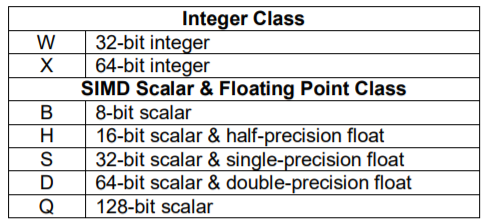
\includegraphics[width=9cm]{figuras/RegisterTable.PNG}
\end{center}
Assim, as instruções podem tomar as seguintes formas:
\begin{center}
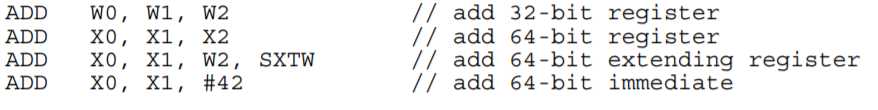
\includegraphics[width=15cm]{RT/figuras/RegisterTypesExample.PNG}
\end{center}

\subsection{Condicionais}
\begin{center}
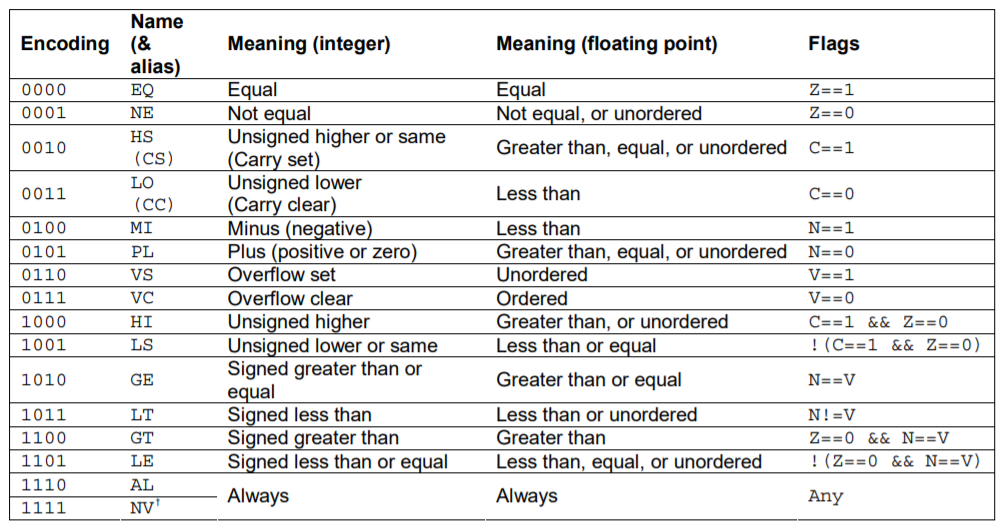
\includegraphics[width=15cm]{figuras/ConditionalIntructionTable.PNG}
\end{center}

\subsection{Usados frequentemente}
As seguintes sintaxes são frequentemente usadas:
\\\\\textbf{Xn -} O operador Xn ou Wn interpreta o registrador 31 como um registrador zero, representado pelos nomes XZR ou WZR respectivamente.
\\\\\textbf{Xn\textbar SP -} O operador Xn\textbar SP ou Wn\textbar WSP interpreta o registrador 31 como o ponteiro de pilha representado pelos nomes SP ou WSP respectivamente.
\\\\\textbf{cond -} Uma condição padrão ARM como EQ, NE, CS\textbar HS, CC\textbar LO, MI, PL, VS, VC, HI, LS, GE, LT, GT, LE, AL ou NV com os mesmos significados da arquitetura AArch32.
\\\\\textbf{invert(cond) -} O inverso de cond, por exemplo, o inverso de GT é LE.
\\\\\textbf{uimmn -} Um n-bit valor imediato sem sinal.
\\\\\textbf{simmn -} Um n-bit valor imediato com sinal em forma de complemento de 2 (onde n inclui o bit de sinal).
\\\\\textbf{label -} Representa uma referência para uma parte do código ou localização.
\\\\\textbf{addr -} Representa um modo de endereçamento.
\\\\\textbf{lshift -} Representa um operador de deslocamento realizado ao final de operadores lógicos. Engloba instruções como LSL, LSR, ASR ou ROR, que são seguidas de uma quantidade constante de deslocamento.
\\\\\textbf{ashift -} Representa um operador de deslocamento realizado ao final de operadores aritiméticos. Engloba instruções como LSL, LSR, ou ASR, que são seguidas de uma quantidade constante e deslocamento.

\subsection{Controle de Fluxo}
\subsubsection{Branch condicional}
Operadores utilizados em branch's condicionais:
\\\\\textbf{B.cond label -} Branch: Condicionalmente salta para label se cond é verdadeiro.
\\\\\textbf{CBNZ Wn, label -} Compare and Branch Not Zero: Condicionalmente salta para label se Wn não é igual a zero.
\\\\\textbf{CBNZ Xn, label -} Compare and Branch Not Zero (extended): Condicionalmente salta para label se Xn não é igual a zero.
\\\\\textbf{CBZ Wn, label -} Compare and Branch Zero: Condicionalmente salta para label se Wn é igual a zero.
\\\\\textbf{CBZ Xn, label -} Compare and Branch Zero (extended): Condicionalmente salta para label se Xn é igual a zero.
\\\\\textbf{TBNZ Xn\textbar Wn \#uimm6 label -} Test and Branch Not Zero: condicionalmente salta para label se o número de bits uimn6 no registrador Xn não é igual a zero.
\\\\\textbf{TBZ Xn\textbar Wn, \#uimm6, label -} Test and Branch Zero: condicionalmente salta para label se o número de bits uimn6 no registrador Xn é igual a zero.

\subsection{Branch não condicional imediato}
Operadores utilizados em branch's não condicionais imediatos:
\\\\\textbf{B label -} Branch: incondicionalmente salta para label. 
\\\\\textbf{BL label -} Branch and Link: incondicionalmente salta para label e escreve o endereço da próxima instrução sequencial no registrador X30.

\subsection{Branch não condicional com registrador}
Operadores utilizados em branch's não condicionais utilizando o endereço de mémoria em registradores:
\\\\\textbf{BLR Xm -} Branch and Link Register: incondicionalmente salta para o endereço em Xm e escreve o endereço da próxima instrução sequencial no registrador X30.
\\\\\textbf{BR Xm -} Branch Register: salta para o endereço em Xm com um lembrete a CPU que isso não é um retorno de subrotina.
\\\\\textbf{RET {Xm} -} Return: salta para o endereço em Xm com um lembrete a CPU que isso é um retorno de subrotina.

\subsection{Memory Access}
\subsubsection{Load-Store com registrador único}
A forma mais geral de load-store, ela suporta uma variedade de modos de endereçamento além dos registradores base Xn ou SP.
\\\\\textbf{LDR Wt, addr -} Load Register: carrega em Wt uma palavra da memória endereçada por addr.
\\\\\textbf{LDR Xt, addr -} Load Register (extended): carrega em Xt uma dupla-palavra (doubleword) da memória endereçada por addr.
\\\\\textbf{LDRB Wt, addr -} Load Byte: carrega em Wt um byte da memória endereçada por addr e preenche os bits restantes com zero.
\\\\\textbf{LDRSB Wt, addr -} Load Signed Byte: carrega em Wt um byte da memória endereçada por addr e preenche os bits restantes de acordo com o sinal.
\\\\\textbf{LDRSB Xt, addr -} Load Signed Byte (extended): carrega em Xt um byte da memória endereçada por addr e preenche os bits restantes de acordo com o sinal do byte.
\\\\\textbf{LDRH Wt, addr -} Load Halfword: carrega em Wt metade de uma palavra (halfword) da memória endereçada por addr e preenche os bits restantes com zero.
\\\\\textbf{LDRSH Wt, addr -} Load Signed Halfword: carrega em Wt metade de uma palavra (halfword) da memória endereçada por addr e preenche os bits restantes de acordo com o sinal.
\\\\\textbf{LDRSH Xt, addr -} Load Signed Halfword (extended): carrega em Xt metade de uma palavra (halfword) da memória endereçada por addr e preenche os bits restantes de acordo com o sinal.
\\\\\textbf{LDRSW Xt, addr -} Load Signed Word (extended): carrega em Xt uma palavra da memória endereçada por addr e preenche os bits restantes de acordo com o sinal.
\\\\\textbf{STR Wt, addr -} Store Register: armazena uma palavra de Wt no endereço de memória addr.
\\\\\textbf{STR Xt, addr -} Store Register (extended): armazena uma palavra dupla (doubleword) de Xt no endereço de memória addr.
\\\\\textbf{STRB Wt, addr -} Store Byte: armazena um byte contido em Wt no endereço de memória addr.
\\\\\textbf{STRH Wt, addr -} Store Halfword: armazena metade de uma palavra (halfword) contida em Wt no endereço de memória addr.

\subsection{Data Processing (immediate)}
Os seguintes grupos de instrução são suportados:
\begin{itemize}
      \item Aritméticas (immediate)
      \item Lógicas (immediate)
      \item Move (immediate)
      \item Bitfield (operations) 
      \item Deslocamento (immediate) 
      \item Extensão de sinal/zero
\end{itemize}
\subsubsection{Arithmetic (immediate)}
Operações aritméticas que aceitam valores imediatos:
\\\\\textbf{ADD Wd\textbar WSP, Wn\textbar WSP, \#aimm -} Add (immediate): Wd\textbar WSP = Wn\textbar WSP + aimm.
\\\\\textbf{ADD Xd\textbar SP, Xn\textbar SP, \#aimm -} Add (extended immediate): Xd\textbar SP = Xn\textbar SP + aimm.
\\\\\textbf{ADDS Wd, Wn\textbar WSP, \#aimm -} Add and set flags (immediate): Wd = Wn\textbar WSP + aimm, configurando as flags de condição.
\\\\\textbf{ADDS Xd, Xn\textbar SP, \#aimm -} Add and set flags (extended immediate): Xd = Xn\textbar SP + aimm, configurando as flags de condição.
\\\\\textbf{SUB Wd\textbar WSP, Wn\textbar WSP, \#aimm -} Subtract (immediate): Wd\textbar WSP = Wn\textbar WSP - aimm.
\\\\\textbf{SUB Xd\textbar SP, Xn\textbar SP, \#aimm -} Subtract (extended immediate): Xd\textbar SP = Xn\textbar SP - aimm.
\\\\\textbf{SUBS Wd, Wn\textbar WSP, \#aimm -} Subtract and set flags (immediate): Wd = Wn\textbar WSP - aimm, configurando as flags de condição.
\\\\\textbf{SUBS Xd, Xn\textbar SP, \#aimm -} Subtract and set flags (extended immediate): Xd = Xn\textbar SP - aimm, configurando as flags de condição.
\\\\\textbf{CMP Wn\textbar WSP, \#aimm -} Compare (immediate): pseudômino para SUBS WZR,Wn\textbar WSP,\#aimm.
\\\\\textbf{CMP Xn\textbarSP, \#aimm -} Compare (extended immediate): pseudômino para SUBS XZR,Xn\textbar SP,\#aimm.
\\\\\textbf{CMN Wn\textbar WSP, \#aimm -} Compare negative (immediate): pseudômino para ADDS WZR,Wn\textbar WSP,\#aimm. 
\\\\\textbf{CMN Xn\textbar SP, \#aimm -} Compare negative (extended immediate): pseudômino para ADDS XZR,Xn\textbar SP,\#aimm. 
\\\\\textbf{MOV Wd\textbar WSP, Wn\textbar WSP -} Move (register): pseudômino para ADD Wd\textbar WSP,Wn\textbar WSP,\#0, mas somente quando algum dos registradores é o WSP. Em outros casos a instrução ORR Wd,WZR,Wn é usada.
\\\\\textbf{MOV Xd\textbar SP, Xn\textbar SP -} Move (extended register): pseudômino para ADD Xd\textbar SP,Xn\textbar SP,\#0, mas somente quando algum dos registradores é o SP. Em outros casos a instrução ORR Xd,XZR,Xn é usada.


\subsubsection{Logical (immediate)}
Operações lógicas que aceitam valores imediatos:
\\\\\textbf{AND Wd\textbar WSP, Wn, \#bimm32 -} Bitwise AND (immediate): Wd\textbar WSP = Wn AND bimm32.
\\\\\textbf{AND Xd\textbar SP, Xn, \#bimm64 -} Bitwise AND (extended immediate): Xd\textbar SP = Xn AND bimm64.
\\\\\textbf{ANDS Wd, Wn, \#bimm32 -} Bitwise AND and Set Flags (immediate): Wd = Wn AND bimm32, atribuindo as flags de condição N e Z baseado no resultado, além de limpar as flags C e V.
\\\\\textbf{ANDS Xd, Xn, \#bimm64 -} Bitwise AND and Set Flags (extended immediate): Xd = Xn AND bimm64, atribuindo as flags de condição N e Z baseado no resultado, além de limpar as flags C e V.
\\\\\textbf{EOR Wd\textbar WSP, Wn, \#bimm32 -} Bitwise exclusive OR (immediate): Wd\textbar WSP = Wn EOR bimm32.
\\\\\textbf{EOR Xd\textbar SP, Xn, \#bimm64 -} Bitwise exclusive OR (extended immediate): Xd\textbar SP = Xn EOR bimm64.
\\\\\textbf{ORR Wd\textbar WSP, Wn, \#bimm32 -} Bitwise inclusive OR (immediate): Wd\textbar WSP = Wn OR bimm32.
\\\\\textbf{ORR Xd\textbar SP, Xn, \#bimm64 -} Bitwise inclusive OR (extended immediate): Xd\textbar SP = Xn OR bimm64.
\\\\\textbf{MOVI Wd, \#bimm32 -} Move bitmask (immediate): pseudômino para ORR Wd,WZR,\#bimm32.
\\\\\textbf{MOVI Xd, \#bimm64 -} Move bitmask (extended immediate): pseudômino para ORR Xd,XZR,\#bimm64.
\\\\\textbf{TST Wn, \#bimm32 -} Bitwise test (immediate): pseudômino para ANDS WZR,Wn,\#bimm32.
\\\\\textbf{TST Xn, \#bimm64 -} Bitwise test (extended immediate): pseudômino para ANDS XZR,Xn,\#bimm64


\subsubsection{Move (wide immediate)}
As seguintes instruções inserem um valor imediato em um registrador destino
\\\\\textbf{MOVZ Wt, \#uimm16{, LSL \#pos} -} Move with Zero (immediate): Wt = LSL(uimm16, pos).
\\\\\textbf{MOVZ Xt, \#uimm16{, LSL \#pos} -} Move with Zero (extended immediate): Xt = LSL(uimm16, pos).
\\\\\textbf{MOVN Wt, \#uimm16{, LSL \#pos} -} Move with NOT (immediate): Wt = NOT(LSL(uimm16, pos)).
\\\\\textbf{MOVN Xt, \#uimm16{, LSL \#pos} -} Move with NOT (extended immediate): Xt = NOT(LSL(uimm16, pos)).
\\\\\textbf{MOVK Wt, \#uimm16{, LSL \#pos} -} Move with Keep (immediate): Wt<pos+15:pos> = uimm16.
\\\\\textbf{MOVK Xt, \#uimm16{, LSL \#pos} -} Move with Keep (extended immediate): Xt<pos+15:pos> = uimm16.
\\\\\textbf{MOV Wd, \#simm32 -} Uma instrução sintética que gera tanto MOVZ, MOVN, como MOVI. 
\\\\\textbf{MOV Xd, \#simm64 -} Funciona assim como o MOV porém para carregar registradores Xd com valores de 64-bit.


\subsection{Bitfield Operations}
Operações de bits:
\\\\\textbf{BFM Wd, Wn, \#r, \#s -} Bitfield Move: se s>=r então Wd<s-r:0> = Wn<s:r>, caso contrário Wd<32+s-r,32-r> = Wn<s:0>. Deixando os outros bits em Wd inalterados.
\\\\\textbf{BFM Xd, Xn, \#r, \#s -} Bitfield Move: se s>=r então Xd<s-r:0> = Xn<s:r>, caso contrário Xd<64+s-r,64-r> = Xn<s:0>. Deixando os outros bits em Xd inalterados.
\\\\\textbf{SBFM Wd, Wn, \#r, \#s -} Signed Bitfield Move: se s>=r então Wd<s-r:0> = Wn<s:r>, caso contrário Wd<32+s-r,32-r> = Wn<s:0>.
atribuindo os bits à esquerda com o valor do bit mais a esquerda e os bits da direita do bitfield de destino com zero.
\\\\\textbf{SBFM Xd, Xn, \#r, \#s -} Signed Bitfield Move: se s>=r então Xd<s-r:0> = Xn<s:r>, caso contrário Xd<64+s-r,64-r> = Xn<s:0>.
atribuindo os bits à esquerda com o valor do bit mais a esquerda e os bits da direita do bitfield de destino com zero.
\\\\\textbf{UBFM Wd, Wn, \#r, \#s -} Unsigned Bitfield Move: se s>=r então Wd<s-r:0> = Wn<s:r>, caso contrário Wd<32+s-r,32-r> = Wn<s:0>.
Atribuindo zero aos bits a esquerda e a direita do bitfield de destino.
\\\\\textbf{UBFM Xd, Xn, \#r, \#s -} Unsigned Bitfield Move: se s>=r então Xd<s-r:0> = Xn<s:r>, caso contrário Xd<32+s-r,32-r> = Xn<s:0>.
Atribuindo zero aos bits a esquerda e a direita do bitfield de destino.
\\\\As seguintes instruções são pseudônimos mais amigáveis para operações de bit:
\\\\\textbf{BFI Wd, Wn, \#lsb, \#width -} Bitfield Insert: pseudônimo para BFM Wd,Wn,\#((32-lsb)\&31),\#(width-1).
\\\\\textbf{BFI Xd, Xn, \#lsb, \#width -} Bitfield Insert (extended): pseudônimo para BFM Xd,Xn,\#((64-lsb)\&63),\#(width-1).
\\\\\textbf{BFXIL Wd, Wn, \#lsb, \#width -} Bitfield Extract and Insert Low: pseudônimo para BFM Wd,Wn,\#lsb,\#(lsb+width-1).
\\\\\textbf{BFXIL Xd, Xn, \#lsb, \#width -} Bitfield Extract and Insert Low (extended): pseudônimo para BFM Xd,Xn,\#lsb,\#(lsb+width-1).
\\\\\textbf{SBFIZ Wd, Wn, \#lsb, \#width -} Signed Bitfield Insert in Zero: pseudônimo para SBFM Wd,Wn,\#((32-lsb)\&31),\#(width-1).
\\\\\textbf{SBFIZ Xd, Xn, \#lsb, \#width -} Signed Bitfield Insert in Zero (extended): pseudônimo para SBFM Xd,Xn,\#((64-lsb)\&63),\#(width-1).
\\\\\textbf{SBFX Wd, Wn, \#lsb, \#width -} Signed Bitfield Extract: pseudônimo para SBFM Wd,Wn,\#lsb,\#(lsb+width-1).
\\\\\textbf{SBFX Xd, Xn, \#lsb, \#width -} Signed Bitfield Extract (extended): pseudônimo para SBFM Xd,Xn,\#lsb,\#(lsb+width-1).
\\\\\textbf{UBFIZ Wd, Wn, \#lsb, \#width -} Unsigned Bitfield Insert in Zero: pseudônimo para UBFM Wd,Wn,\#((32-lsb)\&31),\#(width-1).
\\\\\textbf{UBFIZ Xd, Xn, \#lsb, \#width -} Unsigned Bitfield Insert in Zero (extended): pseudônimo para UBFM Xd,Xn,\#((64-lsb)\&63),\#(width-1).
\\\\\textbf{UBFX Wd, Wn, \#lsb, \#width -} Unsigned Bitfield Extract: pseudônimo para UBFM Wd,Wn,\#lsb,\#(lsb+width-1).
\\\\\textbf{UBFX Xd, Xn, \#lsb, \#width -} Unsigned Bitfield Extract (extended): pseudônimo para UBFM Xd,Xn,\#lsb,\#(lsb+width-1).


\subsubsection{Extract (immediate)}
Operações de extração de bit de valores imediatos:
\\\\\textbf{EXTR Wd, Wn, Wm, \#lsb -} Extract: Wd = Wn:Wm<lsb+31,lsb>. O bit na posição lsb deve estar entre 0 e 31.
\\\\\textbf{EXTR Xd, Xn, Xm, \#lsb -} Extract (extended): Xd = Xn:Xm<lsb+63,lsb>. O bit na posição lsb deve estar entre 0 e 63.


\subsubsection{Shift (immediate)}
a

\\\\\textbf{ASR Wd, Wn, \#uimm -} Arithmetic Shift Right (immediate): alias for SBFM Wd,Wn,\#uimm,\#31. 
\\\\\textbf{ASR Xd, Xn, \#uimm -} Arithmetic Shift Right (extended immediate): alias for SBFM Xd,Xn,\#uimm,\#63. 
\\\\\textbf{LSL Wd, Wn, \#uimm -} Logical Shift Left (immediate): alias for UBFM Wd,Wn,\#((32-uimm)\&31),\#(31-uimm). 
\\\\\textbf{LSL Xd, Xn, \#uimm -} Logical Shift Left (extended immediate): alias for UBFM Xd,Xn,\#((64-uimm)\&63),\#(63-uimm) 
\\\\\textbf{LSR Wd, Wn, \#uimm -} Logical Shift Left (immediate): alias for UBFM Wd,Wn,\#uimm,\#31. 
\\\\\textbf{LSR Xd, Xn, \#uimm -} Logical Shift Left (extended immediate): alias for UBFM Xd,Xn,\#uimm,\#31. 
\\\\\textbf{ROR Wd, Wm, \#uimm -} Rotate Right (immediate): alias for EXTR Wd,Wm,Wm,\#uimm.  
\\\\\textbf{ROR Xd, Xm, \#uimm -} Rotate Right (extended immediate): alias for EXTR Xd,Xm,Xm,\#uimm. 


\subsubsection{Sign/Zero Extend}
\\\\\textbf{SXT[BH] Wd, Wn -} Signed Extend Byte\textbar Halfword: alias for SBFM Wd,Wn,\#0,\#7\textbar 15. 
\\\\\textbf{SXT[BHW] Xd, Wn -} Signed Extend Byte\textbar Halfword\textbar Word (extended): alias for SBFM Xd,Xn,\#0,\#7\textbar 15\textbar 31. 
\\\\\textbf{UXT[BH] Wd, Wn -} Unsigned Extend Byte\textbar Halfword: alias for UBFM Wd,Wn,\#0,\#7\textbar 15. 
\\\\\textbf{UXT[BHW] Xd, Wn -} Unsigned Extend Byte\textbar Halfword\textbar Word (extended): alias for UBFM Xd,Xn,\#0,\#7\textbar 15\textbar 31. 


\subsubsection{Data Processing (register)}
a

\subsubsection{Arithmetic (shifted register)}
\\\\\textbf{ADD Wd, Wn, Wm{, ashift \#imm} -} Add (register): Wd = Wn + ashift(Wm, imm).
\\\\\textbf{ADD Xd, Xn, Xm{, ashift \#imm} -} Add (extended register): Xd = Xn + ashift(Xm, imm). 
\\\\\textbf{ADDS Wd, Wn, Wm{, ashift \#imm} -} Add and Set Flags (register): Wd = Wn + ashift(Wm, imm), setting condition flags. 
\\\\\textbf{ADDS Xd, Xn, Xm{, ashift \#imm} -} Add and Set Flags (extended register): Xd = Xn + ashift(Xm, imm), setting condition flags. 
\\\\\textbf{SUB Wd, Wn, Wm{, ashift \#imm} -} Subtract (register): Wd = Wn - ashift(Wm, imm). 
\\\\\textbf{SUB Xd, Xn, Xm{, ashift \#imm} -} Subtract (extended register): Xd = Xn - ashift(Xm, imm). 
\\\\\textbf{SUBS Wd, Wn, Wm{, ashift \#imm} -} Subtract and Set Flags (register): Wd = Wn - ashift(Wm, imm), setting condition flags. 
\\\\\textbf{SUBS Xd, Xn, Xm{, ashift \#imm} -} Subtract and Set Flags (extended register): Xd = Xn - ashift(Xm, imm), setting condition flags. 
\\\\\textbf{CMN Wn, Wm{, ashift \#imm} -} Compare Negative (register): alias for ADDS WZR, Wn, Wm{, ashift \#imm}. 
\\\\\textbf{CMN Xn, Xm{, ashift \#imm} -} Compare Negative (extended register): alias for ADDS XZR, Xn, Xm{, ashift \#imm}. 

\\\\\textbf{CMP Wn, Wm{, ashift \#imm} -} Compare (register): alias for SUBS WZR, Wn, Wm{,ashift \#imm}. 

\\\\\textbf{CMP Xn, Xm{, ashift \#imm} -} Compare (extended register): alias for SUBS XZR, Xn, Xm{, ashift \#imm}. 

\\\\\textbf{NEG Wd, Wm{, ashift \#imm} -} Negate: alias for SUB Wd, WZR, Wm{, ashift \#imm}. 
\\\\\textbf{NEG Xd, Xm{, ashift \#imm} -} Negate (extended): alias for SUB Xd, XZR, Xm{, ashift \#imm}. 

\\\\\textbf{NEGS Wd, Wm{, ashift \#imm} -} Negate and Set Flags: alias for SUBS Wd, WZR, Wm{, ashift \#imm}. 

\\\\\textbf{NEGS Xd, Xm{, ashift \#imm} -} Negate and Set Flags (extended): alias for SUBS Xd, XZR, Xm{, ashift \#imm}. 



\subsubsection{Arithmetic (extending register)}
a

\\\\\textbf{ADD Wd\textbar WSP, Wn\textbar WSP, Wm, extend {#imm} -} Add (register, extending): Wd\textbar WSP = Wn\textbar WSP + LSL(extend(Wm),imm). 

\\\\\textbf{ADD Xd\textbar SP, Xn\textbar SP, Wm, extend {#imm} -} Add (extended register, extending): Xd\textbar SP = Xn\textbar SP + LSL(extend(Wm),imm). 

\\\\\textbf{ADD Xd\textbar SP, Xn\textbar SP, Xm{, UXTX\textbar LSL \#imm} -} Add (extended register, extending): Xd\textbar SP = Xn\textbar SP + LSL(Xm,imm). 

\\\\\textbf{ADDS Wd, Wn\textbar WSP, Wm, extend {#imm} -} Add and Set Flags (register, extending): Wd = Wn\textbar WSP + LSL(extend(Wm),imm), setting the
condition flags. 
\\\\\textbf{ADDS Xd, Xn\textbar SP, Wm, extend {#imm} -} Add and Set Flags (extended register, extending): Xd = Xn\textbar SP + LSL(extend(Wm),imm), setting
the condition flags. 
\\\\\textbf{ADDS Xd, Xn\textbar SP, Xm{, UXTX\textbar LSL \#imm} -} Add and Set Flags (extended register, extending): Xd = Xn\textbar SP + LSL(Xm,imm), setting the condition
flags. 
\\\\\textbf{SUB Wd\textbar WSP, Wn\textbar WSP, Wm, extend {#imm} -} Subtract (register, extending): Wd\textbar WSP = Wn\textbar WSP - LSL(extend(Wm),imm).

\\\\\textbf{SUB Xd\textbar SP, Xn\textbar SP, Wm, extend {#imm} -} Subtract (extended register, extending): Xd\textbar SP = Xn\textbar SP - LSL(extend(Wm),imm). 

\\\\\textbf{SUB Xd\textbar SP, Xn\textbar SP, Xm{, UXTX\textbar LSL \#imm} -} Subtract (extended register, extending): Xd\textbar SP = Xn\textbar SP - LSL(Xm,imm). 

\\\\\textbf{SUBS Wd, Wn\textbar WSP, Wm, extend {#imm} -} Subtract and Set Flags (register, extending): Wd = Wn\textbar WSP - LSL(extend(Wm),imm), setting the
condition flags. 
\\\\\textbf{SUBS Xd, Xn\textbar SP, Wm, extend {#imm} -} Subtract and Set Flags (extended register, extending): Xd = Xn\textbar SP - LSL(extend(Wm),imm),
setting the condition flags. 
\\\\\textbf{SUBS Xd, Xn\textbar SP, Xm{, UXTX\textbar LSL \#imm} -} Subtract and Set Flags (extended register, extending): Xd = Xn\textbar SP - LSL(Xm,imm), setting the
condition flags. 
\\\\\textbf{CMN Wn\textbar WSP, Wm, extend {#imm} -} Compare Negative (register, extending): alias for ADDS WZR,Wn,Wm,extend {#imm}. 

\\\\\textbf{CMN Xn\textbar SP, Wm, extend {#imm} -} Compare Negative (extended register, extending): alias for ADDS XZR,Xn,Wm,extend {#imm}. 

\\\\\textbf{CMN Xn\textbar SP, Xm{, UXTX\textbar LSL \#imm} -} Compare Negative (extended register, extending): alias for ADDS XZR,Xn,Xm{,UXTX\textbar LSL \#imm}. 

\\\\\textbf{CMP Wn\textbar WSP, Wm, extend {#imm} -} Compare (register, extending): alias for SUBS WZR,Wn,Wm,extend {#imm}. 

\\\\\textbf{CMP Xn\textbar SP, Wm, extend {#imm} -} Compare (extended register, extending): alias for SUBS XZR,Xn,Wm,extend {#imm}. 

\\\\\textbf{CMP Xn\textbar SP, Xm{, UXTX\textbar LSL \#imm} -} Compare (extended register, extending): alias for SUBS XZR,Xn,Xm{,UXTX\textbar LSL \#imm}. 



\subsubsection{Logical (shifted register)}
a

\\\\\textbf{AND Wd, Wn, Wm{, lshift \#imm} -} Bitwise AND (register): Wd = Wn AND lshift(Wm, imm). 

\\\\\textbf{AND Xd, Xn, Xm{, lshift \#imm} -} Bitwise AND (extended register): Xd = Xn AND lshift(Xm, imm). 

\\\\\textbf{ANDS Wd, Wn, Wm{, lshift \#imm} -} Bitwise AND and Set Flags (register): Wd = Wn AND lshift(Wm, imm), setting N \& Z condition flags
based on the result and clearing the C \& V flags. 
\\\\\textbf{ANDS Xd, Xn, Xm{, lshift \#imm} -} Bitwise AND and Set Flags (extended register): Xd = Xn AND lshift(Xm, imm), setting N \& Z
condition flags based on the result and clearing the C \& V flags. 

\\\\\textbf{BIC Wd, Wn, Wm{, lshift \#imm} -} Bit Clear (register): Wd = Wn AND NOT(lshift(Wm, imm)). 

\\\\\textbf{BIC Xd, Xn, Xm{, lshift \#imm} -} Bit Clear (extended register): Xd = Xn AND NOT(lshift(Xm, imm)). 
\\\\\textbf{BICS Wd, Wn, Wm{, lshift \#imm} -} Bit Clear and Set Flags (register): Wd = Wn AND NOT(lshift(Wm, imm)), setting N \& Z condition
flags based on the result and clearing the C \& V flags. 
\\\\\textbf{BICS Xd, Xn, Xm{, lshift \#imm} -} Bit Clear and Set Flags (extended register): Xd = Xn AND NOT(lshift(Xm, imm)), setting N \& Z
condition flags based on the result and clearing the C \& V flags. 
\\\\\textbf{EON Wd, Wn, Wm{, lshift \#imm} -} Bitwise exclusive OR NOT (register): Wd = Wn EOR NOT(lshift(Wm, imm)). 

\\\\\textbf{EON Xd, Xn, Xm{, lshift \#imm} -} Bitwise exclusive OR NOT (extended register): Xd = Xn EOR NOT(lshift(Xm, imm)). 

\\\\\textbf{EOR Wd, Wn, Wm{, lshift \#imm} -} Bitwise exclusive OR (register): Wd = Wn EOR lshift(Wm, imm). 

\\\\\textbf{EOR Xd, Xn, Xm{, lshift \#imm} -} Bitwise exclusive OR (extended register): Xd = Xn EOR lshift(Xm, imm). 

\\\\\textbf{ORR Wd, Wn, Wm{, lshift \#imm} -} Bitwise inclusive OR (register): Wd = Wn OR lshift(Wm, imm). 
\\\\\textbf{ORR Xd, Xn, Xm{, lshift \#imm} -} Bitwise inclusive OR (extended register): Xd = Xn OR lshift(Xm, imm). 

\\\\\textbf{ORN Wd, Wn, Wm{, lshift \#imm} -} Bitwise inclusive OR NOT (register): Wd = Wn OR NOT(lshift(Wm, imm)). 

\\\\\textbf{ORN Xd, Xn, Xm{, lshift \#imm} -} Bitwise inclusive OR NOT (extended register): Xd = Xn OR NOT(lshift(Xm, imm)). 

\\\\\textbf{MOV Wd, Wm -} Move (register): alias for ORR Wd,WZR,Wm. 

\\\\\textbf{MOV Xd, Xm -} Move (extended register): alias for ORR Xd,XZR,Xm. 

\\\\\textbf{MVN Wd, Wm{, lshift \#imm} -} Move NOT (register): alias for ORN Wd,WZR,Wm{,lshift \#imm}. 
\\\\\textbf{MVN Xd, Xm{, lshift \#imm} -} Move NOT (extended register): alias for ORN Xd,XZR,Xm{,lshift \#imm}. 

\\\\\textbf{TST Wn, Wm{, lshift \#imm} -} Bitwise Test (register): alias for ANDS WZR,Wn,Wm{,lshift \#imm}. 

\\\\\textbf{TST Xn, Xm{, lshift \#imm} -} Bitwise Test (extended register): alias for ANDS XZR,Xn,Xm{,lshift \#imm}. 


\subsubsection{Variable Shift}
a

\\\\\textbf{ASRV Wd, Wn, Wm -} Arithmetic Shift Right Variable: Wd = ASR(Wn, Wm \& 0x1f).
\\\\\textbf{ASRV Xd, Xn, Xm -} Arithmetic Shift Right Variable (extended): Xd = ASR(Xn, Xm \& 0x3f). 

\\\\\textbf{LSLV Wd, Wn, Wm -} Logical Shift Left Variable: Wd = LSL(Wn, Wm \& 0x1f). 

\\\\\textbf{LSLV Xd, Xn, Xm -} Logical Shift Left Variable (extended register): Xd = LSL(Xn, Xm \& 0x3f). 

\\\\\textbf{LSRV Wd, Wn, Wm -} Logical Shift Right Variable: Wd = LSR(Wn, Wm \& 0x1f). 

\\\\\textbf{LSRV Xd, Xn, Xm -} Logical Shift Right Variable (extended): Xd = LSR(Xn, Xm \& 0x3f). 

\\\\\textbf{RORV Wd, Wn, Wm -} Rotate Right Variable: Wd = ROR(Wn, Wm \& 0x1f). 

\\\\\textbf{RORV Xd, Xn, Xm -} Rotate Right Variable (extended): Xd = ROR(Xn, Xm \& 0x3f). 

a

\\\\\textbf{ASR Wd, Wn, Wm -} Arithmetic Shift Right (register): preferred alias for ASRV Wd, Wn, Wm. 

\\\\\textbf{ASR Xd, Xn, Xm -} Arithmetic Shift Right (extended register): preferred alias for ASRV Xd, Xn, Xm. 

\\\\\textbf{LSL Wd, Wn, Wm -} Logical Shift Left (register): preferred alias for LSLV Wd, Wn, Wm. 

\\\\\textbf{LSL Xd, Xn, Xm -} Logical Shift Left (extended register): preferred alias for LSLV Xd, Xn, Xm. 

\\\\\textbf{LSR Wd, Wn, Wm -} Logical Shift Right (register): preferred alias for LSRV Wd, Wn, Wm. 

\\\\\textbf{LSR Xd, Xn, Xm -} Logical Shift Right (extended register): preferred alias for LSRV Xd, Xn, Xm. 
\\\\\textbf{ROR Wd, Wn, Wm -} Rotate Right (register): preferred alias for RORV Wd, Wn, Wm. 

\\\\\textbf{ROR Xd, Xn, Xm -} Rotate Right (extended register): preferred alias for RORV Xd, Xn, Xm. 


\subsubsection{Bit Operations}

\\\\\textbf{CLS Wd, Wm -} Count Leading Sign Bits: sets Wd to the number of consecutive bits following the topmost bit in Wm, that
are the same as the topmost bit. The count does not include the topmost bit itself, so the result will be in
the range 0 to 31 inclusive.
\\\\\textbf{CLS Xd, Xm -} Count Leading Sign Bits (extended): sets Xd to the number of consecutive bits following the topmost bit
in Xm, that are the same as the topmost bit. The count does not include the topmost bit itself, so the result
will be in the range 0 to 63 inclusive. 
\\\\\textbf{CLZ Wd, Wm -} Count Leading Zeros: sets Wd to the number of binary zeros at the most significant end of Wm. The result
will be in the range 0 to 32 inclusive. 
\\\\\textbf{CLZ Xd, Xm -} Count Leading Zeros: (extended) sets Xd to the number of binary zeros at the most significant end of Xm.
The result will be in the range 0 to 64 inclusive. 
\\\\\textbf{RBIT Wd, Wm -} Reverse Bits: reverses the 32 bits from Wm, writing to Wd. 

\\\\\textbf{RBIT Xd, Xm -} Reverse Bits (extended): reverses the 64 bits from Xm, writing to Xd. 

\\\\\textbf{REV Wd, Wm -} Reverse Bytes: reverses the 4 bytes in Wm, writing to Wd. 

\\\\\textbf{REV Xd, Xm -} Reverse Bytes (extended): reverses 8 bytes in Xm, writing to Xd. 

\\\\\textbf{REV16 Wd, Wm -} Reverse Bytes in Halfwords: reverses the 2 bytes in each 16-bit element of Wm, writing to Wd. 

\\\\\textbf{REV16 Xd, Xm -} Reverse Bytes in Halfwords (extended): reverses the 2 bytes in each 16-bit element of Xm, writing to Xd. 

\\\\\textbf{REV32 Xd, Xm -} Reverse Bytes in Words (extended): reverses the 4 bytes in each 32-bit element of Xm, writing to Xd. 


\subsubsection{Conditional Data Processing}
a

\\\\\textbf{ADC Wd, Wn, Wm -} Add with Carry: Wd = Wn + Wm + C. 

\\\\\textbf{ADC Xd, Xn, Xm -} Add with Carry (extended): Xd = Xn + Xm + C. 
\\\\\textbf{ADCS Wd, Wn, Wm -} Add with Carry and Set Flags: Wd = Wn + Wm + C, setting the condition flags. 

\\\\\textbf{ADCS Xd, Xn, Xm -} Add with Carry and Set Flags (extended): Xd = Xn + Xm + C, setting the condition flags. 

\\\\\textbf{CSEL Wd, Wn, Wm, cond -} Conditional Select: Wd = if cond then Wn else Wm.

\\\\\textbf{CSEL Xd, Xn, Xm, cond -} Conditional Select (extended): Xd = if cond then Xn else Xm. 

\\\\\textbf{CSINC Wd, Wn, Wm, cond -} Conditional Select Increment: Wd = if cond then Wn else Wm+1. 

\\\\\textbf{CSINC Xd, Xn, Xm, cond -} Conditional Select Increment (extended): Xd = if cond then Xn else Xm+1. 

\\\\\textbf{CSINV Wd, Wn, Wm, cond -} Conditional Select Invert: Wd = if cond then Wn else NOT(Wm). 

\\\\\textbf{CSINV Xd, Xn, Xm, cond -} Conditional Select Invert (extended): Xd = if cond then Xn else NOT(Xm). 

\\\\\textbf{CSNEG Wd, Wn, Wm, cond -} Conditional Select Negate: Wd = if cond then Wn else -Wm. 

\\\\\textbf{CSNEG Xd, Xn, Xm, cond -} Conditional Select Negate (extended): Xd = if cond then Xn else -Xm. 

\\\\\textbf{CSET Wd, cond -} Conditional Set: Wd = if cond then 1 else 0.
Alias for CSINC Wd,WZR,WZR,invert(cond). 
\\\\\textbf{CSET Xd, cond -} Conditional Set (extended): Xd = if cond then 1 else 0.
Alias for CSINC Xd,XZR,XZR,invert(cond)
\\\\\textbf{CSETM Wd, cond -} Conditional Set Mask: Wd = if cond then -1 else 0.
Alias for CSINV Wd,WZR,WZR,invert(cond).
\\\\\textbf{CSETM Xd, cond -} Conditional Set Mask (extended): Xd = if cond then -1 else 0.
Alias for CSINV Xd,WZR,WZR,invert(cond). 
\\\\\textbf{CINC Wd, Wn, cond -} Conditional Increment: Wd = if cond then Wn+1 else Wn.
Alias for CSINC Wd,Wn,Wn,invert(cond).
\\\\\textbf{CINC Xd, Xn, cond -} Conditional Increment (extended): Xd = if cond then Xn+1 else Xn.
Alias for CSINC Xd,Xn,Xn,invert(cond). 
\\\\\textbf{CINV Wd, Wn, cond -} Conditional Invert: Wd = if cond then NOT(Wn) else Wn.
Alias for CSINV Wd,Wn,Wn,invert(cond).
\\\\\textbf{CINV Xd, Xn, cond -} Conditional Invert (extended): Xd = if cond then NOT(Xn) else Xn.
Alias for CSINV Xd,Xn,Xn,invert(cond). 
\\\\\textbf{CNEG Wd, Wn, cond -} Conditional Negate: Wd = if cond then -Wn else Wn.
Alias for CSNEG Wd,Wn,Wn,invert(cond).
\\\\\textbf{CNEG Xd, Xn, cond -} Conditional Negate (extended): Xd = if cond then -Xn else Xn.
Alias for CSNEG Xd,Xn,Xn,invert(cond). 
\\\\\textbf{SBC Wd, Wn, Wm -} Subtract with Carry: Wd = Wn - Wm - 1 + C. 

\\\\\textbf{SBC Xd, Xn, Xm -} Subtract with Carry (extended): Xd = Xn - Xm - 1 + C. 

\\\\\textbf{SBCS Wd, Wn, Wm -} Subtract with Carry and Set Flags: Wd = Wn - Wm - 1 + C , setting the condition flags. 

\\\\\textbf{SBCS Xd, Xn, Xm -} Subtract with Carry and Set Flags (extended): Xd = Xn - Xm - 1 + C , setting the condition flags. 

\\\\\textbf{NGC Wd, Wm -} Negate with Carry: Wd = -Wm - 1 + C.
Alias for SBC Wd,WZR,Wm.

\\\\\textbf{NGC Xd, Xm -} Negate with Carry (extended): Xd = -Xm - 1 + C.
Alias for SBC Xd,XZR,Xm.

\\\\\textbf{NGCS Wd, Wm -} Negate with Carry and Set Flags: Wd = -Wm - 1 + C, setting the condition flags.
Alias for SBCS Wd,WZR,Wm.

\\\\\textbf{NGCS Xd, Xm -} Negate with Carry and Set Flags (extended): Xd = -Xm - 1 + C, setting the condition flags.
Alias for SBCS Xd,XZR,Xm.


\subsubsection{Conditional Comparison}
a

\\\\\textbf{CCMN Wn, Wm, \#uimm4, cond -} Conditional Compare Negative (register):
NZCV = if cond then CMP(Wn,-Wm) else uimm4. 
\\\\\textbf{CCMN Xn, Xm, \#uimm4, cond -} Conditional Compare Negative (extended register):
NZCV = if cond then CMP(Xn,-Xm) else uimm4. 
\\\\\textbf{CCMN Wn, \#uimm5, \#uimm4, cond -} Conditional Compare Negative (immediate):
NZCV = if cond then CMP(Wn,-uimm5) else uimm4. 
\\\\\textbf{CCMN Xn, \#uimm5, \#uimm4, cond -} Conditional Compare Negative (extended immediate):
NZCV = if cond then CMP(Xn,-uimm5) else uimm4.
\\\\\textbf{CCMP Wn, Wm, \#uimm4, cond -} Conditional Compare (register):
NZCV = if cond then CMP(Wn,Wm) else uimm4. 

\\\\\textbf{CCMP Xn, Xm, \#uimm4, cond -} Conditional Compare (extended register):
NZCV = if cond then CMP(Xn,Xm) else uimm4. 
\\\\\textbf{CCMP Wn, \#uimm5, \#uimm4, cond -} Conditional Compare (immediate):
NZCV = if cond then CMP(Wn,uimm5) else uimm4. 
\\\\\textbf{CCMP Xn, \#uimm5, \#uimm4, cond -} Conditional Compare (extended immediate):
NZCV = if cond then CMP(Xn,uimm5) else uimm4.


\subsection{Integer Multiply / Divide}

\subsubsection{Multiply}

\\\\\textbf{MADD Wd, Wn, Wm, Wa -} Multiply-Add: Wd = Wa + (Wn × Wm). 

\\\\\textbf{MADD Xd, Xn, Xm, Xa -} Multiply-Add (extended): Xd = Xa + (Xn × Xm.) 

\\\\\textbf{MSUB Wd, Wn, Wm, Wa -} Multiply-Subtract: Wd = Wa – (Wn × Wm). 

\\\\\textbf{MSUB Xd, Xn, Xm, Xa -} Multiply-Subtract (extended): Xd = Xa – (Xn × Xm). 

\\\\\textbf{MNEG Wd, Wn, Wm -} Multiply-Negate: Wd = –(Wn × Wm).
Alias for MSUB Wd, Wn, Wm, WZR. 
\\\\\textbf{MNEG Xd, Xn, Xm -} Multiply-Negate (extended): Xd = –(Xn × Xm).
Alias for MSUB Xd, Xn, Xm, XZR. 
\\\\\textbf{MUL Wd, Wn, Wm -} Multiply: Wd = Wn × Wm.
Alias for MADD Wd, Wn, Wm, WZR. 
\\\\\textbf{MUL Xd, Xn, Xm -} Multiply (extended): Xd = Xn × Xm.
Alias for MADD Xd, Xn, Xm, XZR. 
\\\\\textbf{SMADDL Xd, Wn, Wm, Xa -} Signed Multiply-Add Long: Xd = Xa + (Wn × Wm), treating source operands as signed. 
\\\\\textbf{SMSUBL Xd, Wn, Wm, Xa -} Signed Multiply-Subtract Long: Xd = Xa – (Wn × Wm), treating source operands as signed. 

\\\\\textbf{SMNEGL Xd, Wn, Wm -} Signed Multiply-Negate Long: Xd = -(Wn × Wm), treating source operands as signed.
Alias for SMSUBL Xd, Wn, Wm, XZR.
\\\\\textbf{SMULL Xd, Wn, Wm -} Signed Multiply Long: Xd = Wn × Wm, treating source operands as signed.
Alias for SMADDL Xd, Wn, Wm, XZR.
\\\\\textbf{SMULH Xd, Xn, Xm -} Signed Multiply High: Xd = (Xn × Xm)<127:64>, treating source operands as signed. 

\\\\\textbf{UMADDL Xd, Wn, Wm, Xa -} Unsigned Multiply-Add Long: Xd = Xa + (Wn × Wm), treating source operands as unsigned. 

\\\\\textbf{UMSUBL Xd, Wn, Wm, Xa -} Unsigned Multiply-Subtract Long: Xd = Xa – (Wn × Wm), treating source operands as unsigned. 

\\\\\textbf{UMNEGL Xd, Wn, Wm -} Unsigned Multiply-Negate Long: Xd = -(Wn × Wm), treating source operands as unsigned.
Alias for UMSUBL Xd, Wn, Wm, XZR.
\\\\\textbf{UMULL Xd, Wn, Wm -} Unsigned Multiply Long: Xd = Wn × Wm, treating source operands as unsigned.
Alias for UMADDL Xd, Wn, Wm, XZR
\\\\\textbf{UMULH Xd, Xn, Xm -} Unsigned Multiply High: Xd = (Xn × Xm)<127:64>, treating source operands as unsigned. 


\subsubsection{Divide}
a

\\\\\textbf{SDIV Wd, Wn, Wm -} Signed Divide: Wd = Wn ÷ Wm, treating source operands as signed. 

\\\\\textbf{SDIV Xd, Xn, Xm -} Signed Divide (extended): Xd = Xn ÷ Xm, treating source operands as signed. 

\\\\\textbf{UDIV Wd, Wn, Wm -} Unsigned Divide: Wd = Wn ÷ Wm, treating source operands as unsigned. 

\\\\\textbf{UDIV Xd, Xn, Xm -} Unsigned Divide (extended): Xd = Xn ÷ Xm, treating source operands as unsigned. 

\section{Detalhes da Arquitetura}
    \subsection{Tipo de Arquitetura}
        A arquitetura ARMv8-A extende a arquitetura ARMv7, tendo agora dois estados de execução: 32 bits e 64 bits, mantendo a compatibilidade com a arquitetura predecessora e, portanto, seus fundamentos.
        A arquitetura ARMv8-A segue uma pipeline, com a quantidade de estágios variando de acordo com o processador em que a arquitetura foi implementada. A ordem de execução também varia de acordo com o processador, como exemplo:
        \begin{itemize}
            \item Cortex-A53: Pipeline executa em ordem.
        \end{itemize}
        \begin{itemize}
            \item Cortex-A57: Superescalar, não segue uma ordem específica (Speculative Issue).
        \end{itemize}

    \subsection{Arquitetura do Processador}
        Exemplificaremos a implementação da arquitetura ARMv8-A em um processador Cortex-A57, lançado em janeiro de 2015, com uma quantidade de cores que varia de 1 à 4.
        \begin{itemize}
            \item Estágios por Pipeline: 15+.
        \end{itemize}
        \begin{itemize}
            \item Velocidade do Clock: 1.5 à 2.5 GHz em 20nm.
        \end{itemize}
        \begin{itemize}
            \item Tamanho do Cache L1 (Instrução): 48 KB (associativo de 3 vias).
        \end{itemize}
        \begin{itemize}
            \item Tamanho do Cache L1 (Dados): 32 KB (associativo bidirecional).
        \end{itemize}
        \begin{itemize}
            \item Tamanho do Cache L2: 512 KB à 2 MB (associativo de 16 vias).
        \end{itemize}
        \begin{itemize}
            \item Taxa de Tranferência máxima de Inteiro: 4.1 à 4.76MIPS/MHz
        \end{itemize}        
    
\bibliographystyle{ppgsi}
\bibliography{bibitex}
\nocite{manual}
\nocite{pressreal}
\nocite{pressarmv86}
\nocite{pressSdragon}
\nocite{bench}
\nocite{atomclose}

\end{document}
